\documentclass{article}
\usepackage{graphicx} % Required for inserting images
\usepackage{float}
\usepackage[T1]{fontenc}
\usepackage{amsmath}
\usepackage[margin=1in]{geometry}
\usepackage{booktabs}
\usepackage{tabularx}
\usepackage[hidelinks]{hyperref}

\title{Skew at entry and the choice of put strike}
\author{Diagnostic \textperiodcentered{} L/S Gamma Desk, QUANTT}
\date{2026-11-02}

\begin{document}

\maketitle

\textbf{Question:} On the 35\% stress-sized put book, does put skew at entry change which put to sell, so that ``sell a lower delta when skew is steep, 25-delta when it is flat'' (or the reverse) would have helped? And does skew predict the book's P\&L beyond what the implied-vol level already says?

\textbf{Method:}

\begin{itemize}

\item \textbf{No new trials.} This note uses only registered runs and the v1 replay snapshots, development window 2014-06-02 to 2024-12-31:

\begin{itemize}

\item 25-delta: the 2026-10-22 \texttt{hedged} book;

\item 20- and 15-delta: \texttt{put20} and \texttt{put15} from the 2026-11-02 lower-delta card.

\end{itemize}

Each book has 1x and 2x spread runs. The 2x runs are a check.

\item \textbf{Skew:} for each round trip, the 25-delta put IV minus the ATM (50-delta) put IV on the traded expiry. Both IVs are interpolated on |delta| in the decision chain the engine read at entry, and the result is in vol points.

\item \textbf{Terciles:} cut points come from all entries of the three 1x books pooled (373 distinct entries):

\begin{itemize}

\item flat: below 2.42 points;

\item steep: above 3.33 points;

\item median: 2.74 points.

\end{itemize}

\item \textbf{Measure:} net P\&L per contract per round trip (net of commissions and spreads, including the hedge), shown as mean, standard error, count, and dollar sum. Aggregates only.

\item \textbf{Matched days:} round trips that two books entered at the same time, which isolates the strike from the roll calendar.

\end{itemize}

\section{Short answer}

\begin{itemize}

\item \textbf{Skew sorts P\&L, but mostly as a proxy for the vol level.}

\begin{itemize}

\item Entries in the flat-skew tercile lost money per contract at every delta, while the middle and steep terciles made money.

\item Skew moves with ATM IV (correlation 0.77), and beyond what ATM IV implies it sorts P\&L only weakly. That fits the desk's reading of Kozhan et al. (2013): skew is mostly the same bet as variance.

\end{itemize}

\item \textbf{The best strike doesn't change with skew.} On days when two books entered together, the 20- and 25-delta puts earned about the same per contract in every skew tercile. The 15-delta put trailed the 25-delta in every tercile. Neither ``lower delta when steep'' nor the reverse is supported.

\item \textbf{It doesn't justify a strike-choice card.} The one stable pattern, that flat-skew (low-IV) entries lose, is a vol-level gate. Gates have failed on this desk three times. A suggested bar is below if the PM wants to test it anyway.

\end{itemize}

\section{Skew and P\&L by strike}

Net P\&L per contract per round trip, 1x spreads, full window. Each cell is mean (standard error), with the count and dollar sum in the last two columns.

\begin{center}\small
\begin{tabularx}{\linewidth}{l >{\raggedright\arraybackslash}X >{\raggedright\arraybackslash}X >{\raggedright\arraybackslash}X >{\raggedright\arraybackslash}X >{\raggedright\arraybackslash}X}
\toprule
\textbf{Delta} & \textbf{Flat skew} & \textbf{Middle} & \textbf{Steep skew} & \textbf{Count (flat /\allowbreak{} mid /\allowbreak{} steep)} & \textbf{Dollar sum (flat /\allowbreak{} mid /\allowbreak{} steep)} \\
\midrule
25 & \ensuremath{-}\$22.8 (\$21.3) & \$14.3 (\$17.3) & \$39.1 (\$27.5) & 61 /\allowbreak{} 59 /\allowbreak{} 62 & \ensuremath{-}\$16.9k /\allowbreak{} \$28.9k /\allowbreak{} \$101.2k \\
20 & \ensuremath{-}\$15.4 (\$16.4) & \$36.1 (\$9.5) & \$45.0 (\$17.1) & 64 /\allowbreak{} 58 /\allowbreak{} 70 & \ensuremath{-}\$14.8k /\allowbreak{} \$51.6k /\allowbreak{} \$108.5k \\
15 & \ensuremath{-}\$16.5 (\$16.4) & \$29.7 (\$11.3) & \$24.6 (\$18.9) & 62 /\allowbreak{} 63 /\allowbreak{} 69 & \ensuremath{-}\$17.7k /\allowbreak{} \$43.8k /\allowbreak{} \$74.9k \\
\bottomrule
\end{tabularx}
\end{center}

\begin{figure}[H]\centering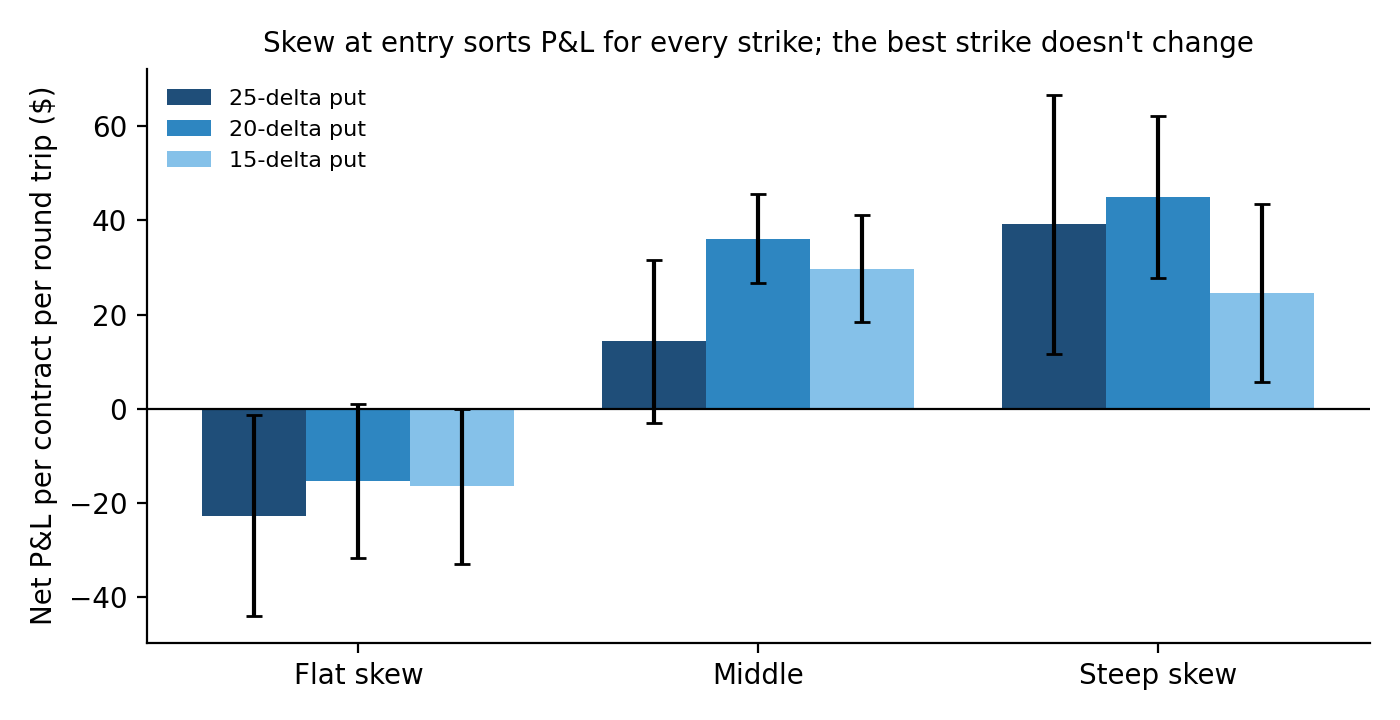
\includegraphics[width=0.92\linewidth]{2026-11-02-skew-and-strike.png}\caption{Net P\&L per contract per round trip by skew tercile at entry, 1x spreads, 2014-06 to 2024-12. Whiskers are \ensuremath{\pm}1 standard error.}\end{figure}

\subsection{The pattern holds across halves and without the two big episodes}

Mean net P\&L per contract, 1x (flat /\allowbreak{} middle /\allowbreak{} steep):

\begin{center}\small
\begin{tabularx}{\linewidth}{>{\raggedright\arraybackslash}X >{\raggedright\arraybackslash}X >{\raggedright\arraybackslash}X >{\raggedright\arraybackslash}X}
\toprule
\textbf{Sample} & \textbf{25-delta} & \textbf{20-delta} & \textbf{15-delta} \\
\midrule
2014-2019 & \ensuremath{-}\$5.1 /\allowbreak{} \$21.3 /\allowbreak{} \$30.8 & \ensuremath{-}\$18.3 /\allowbreak{} \$24.8 /\allowbreak{} \$31.8 & \ensuremath{-}\$23.5 /\allowbreak{} \$25.7 /\allowbreak{} \$11.1 \\
2020-2024 & \ensuremath{-}\$45.0 /\allowbreak{} \ensuremath{-}\$1.6 /\allowbreak{} \$43.4 & \ensuremath{-}\$10.9 /\allowbreak{} \$59.3 /\allowbreak{} \$53.2 & \ensuremath{-}\$6.2 /\allowbreak{} \$38.9 /\allowbreak{} \$32.8 \\
Without 19 Feb-30 Apr 2020 & \ensuremath{-}\$15.9 /\allowbreak{} \$14.3 /\allowbreak{} \$53.1 & \ensuremath{-}\$15.4 /\allowbreak{} \$36.1 /\allowbreak{} \$49.2 & \ensuremath{-}\$16.5 /\allowbreak{} \$29.7 /\allowbreak{} \$33.9 \\
Without August 2015 & \ensuremath{-}\$22.8 /\allowbreak{} \$18.1 /\allowbreak{} \$37.9 & \ensuremath{-}\$15.4 /\allowbreak{} \$38.9 /\allowbreak{} \$42.7 & \ensuremath{-}\$14.9 /\allowbreak{} \$29.5 /\allowbreak{} \$22.9 \\
Without both & \ensuremath{-}\$15.9 /\allowbreak{} \$18.1 /\allowbreak{} \$52.1 & \ensuremath{-}\$15.4 /\allowbreak{} \$38.9 /\allowbreak{} \$46.9 & \ensuremath{-}\$14.9 /\allowbreak{} \$29.5 /\allowbreak{} \$32.3 \\
2x spreads, full window & \ensuremath{-}\$28.2 /\allowbreak{} \$9.3 /\allowbreak{} \$34.8 & \ensuremath{-}\$20.8 /\allowbreak{} \$33.4 /\allowbreak{} \$41.4 & \ensuremath{-}\$18.3 /\allowbreak{} \$29.0 /\allowbreak{} \$28.6 \\
\bottomrule
\end{tabularx}
\end{center}

The flat tercile is negative in every row and at every delta. The rank correlation between skew and per-contract P\&L is 0.22-0.28 across the three books. A trip is dropped from the ``without'' rows if it was open at any time in the excluded window.

\section{Skew is mostly the vol level}

\begin{itemize}

\item \textbf{Skew tracks ATM IV.} Across the 373 entries, skew correlates 0.77 with ATM IV and 0.31 with VRP. A linear fit gives skew \ensuremath{\approx} 0.18 \ensuremath{\times} ATM IV + 0.3 points.

\begin{itemize}

\item Median skew by year ranged from 1.8 points (2024) to 4.6 points (2020).

\item So the flat tercile is mostly the calm, low-IV entries. The 2026-10-22 card had already found that entries below 15\% IV lost money.

\end{itemize}

\item \textbf{ATM IV alone sorts P\&L about as well.} Mean per contract at 1x, by ATM IV tercile (low /\allowbreak{} mid /\allowbreak{} high, cut at 11.9\% and 17.3\%):

\begin{itemize}

\item 25-delta: \ensuremath{-}\$19.3 /\allowbreak{} \$26.1 /\allowbreak{} \$26.0;

\item 20-delta: \ensuremath{-}\$9.1 /\allowbreak{} \$17.3 /\allowbreak{} \$60.3;

\item 15-delta: \ensuremath{-}\$2.3 /\allowbreak{} \$6.7 /\allowbreak{} \$36.7.

\end{itemize}

\item \textbf{Skew beyond the IV level adds little.}

\begin{itemize}

\item Terciles of skew after removing the fitted ATM IV part, flat /\allowbreak{} mid /\allowbreak{} steep:

\begin{itemize}

\item 25-delta: \$11.3 /\allowbreak{} \ensuremath{-}\$2.3 /\allowbreak{} \$20.3;

\item 20-delta: \$12.7 /\allowbreak{} \$8.8 /\allowbreak{} \$43.9;

\item 15-delta: \$12.8 /\allowbreak{} \$12.7 /\allowbreak{} \$13.8.

\end{itemize}

\item In a regression of per-contract P\&L on skew and ATM IV, the skew coefficient is significant only for the 20-delta book (t = 2.1). It is insignificant for 25-delta (t = 0.8) and negative for 15-delta (t = \ensuremath{-}0.5). With three books tested, one t of 2.1 is weak evidence.

\end{itemize}

\item \textbf{This matches the literature the desk already cites.} The 2026-10-31 signals report notes that Kozhan, Neuberger \& Schneider (2013) find skew and variance premia are largely one risk, and that skew trades are mostly the same bet as VRP. Our data agree in direction: the skew effect here is mostly the IV-level effect.

\end{itemize}

\section{Does the best strike change with skew?}

Matched entries are round trips two books opened at the same time. The table gives the mean per-contract difference, with the standard error in brackets, by skew tercile.

\begin{center}\small
\begin{tabularx}{\linewidth}{l l >{\raggedright\arraybackslash}X >{\raggedright\arraybackslash}X l >{\raggedright\arraybackslash}X >{\raggedright\arraybackslash}X}
\toprule
\textbf{Comparison} & \textbf{Spread} & \textbf{Matched trips} & \textbf{Flat} & \textbf{Middle} & \textbf{Steep} & \textbf{All} \\
\midrule
20 minus 25 & 1x & 92 & +\$8.3 (\$9.1) & \ensuremath{-}\$5.4 (\$3.3) & \ensuremath{-}\$1.0 (\$5.9) & +\$1.0 (\$4.0) \\
20 minus 25 & 2x & 87 & +\$13.3 (\$10.6) & \ensuremath{-}\$4.0 (\$5.6) & \ensuremath{-}\$1.7 (\$6.0) & +\$2.7 (\$4.6) \\
15 minus 25 & 1x & 61 & \ensuremath{-}\$26.2 (\$10.4) & \ensuremath{-}\$7.1 (\$8.1) & \ensuremath{-}\$22.9 (\$14.9) & \ensuremath{-}\$18.6 (\$7.2) \\
15 minus 25 & 2x & 66 & \ensuremath{-}\$23.0 (\$9.3) & \ensuremath{-}\$9.7 (\$8.1) & \ensuremath{-}\$24.5 (\$15.3) & \ensuremath{-}\$18.7 (\$6.7) \\
15 minus 20 & 1x & 91 & +\$2.2 (\$4.1) & \ensuremath{-}\$1.4 (\$4.0) & \ensuremath{-}\$38.3 (\$20.2) & \ensuremath{-}\$15.8 (\$8.8) \\
\bottomrule
\end{tabularx}
\end{center}

\begin{itemize}

\item \textbf{20 vs 25:} no difference that survives the standard errors. On the 92 matched days the two books made about the same:

\begin{itemize}

\item net: \$70.0k for the 20-delta book against \$71.7k;

\item per contract: \$31.0 against \$31.2.

\end{itemize}

The flat-tercile edge for the 20-delta put (+\$8 at 1x, +\$13 at 2x) is about one standard error and has no partner in the other terciles.

\item \textbf{15 vs 25:} the 15-delta put trailed in every tercile, by about \$19 per contract overall. The gap is largest when skew is flat or steep, not when it is steep alone.

\item \textbf{15 vs 20:} the gap is concentrated in the steep tercile (\ensuremath{-}\$38, standard error \$20). That is the opposite of ``sell further out when skew is steep''.

\item \textbf{Neither rule would have helped:} not ``lower delta when skew is steep, 25-delta when flat'', and not its reverse. The lower-delta card's lead for \texttt{put20} came from re-entering on different days (mostly August 2015), not from the strike. The matched-day results here confirm that.

\end{itemize}

\section{Does it justify a card?}

Not a strike-choice card: the best delta doesn't change with skew in the matched comparison.

The only stable pattern is that flat-skew entries lose. That is mostly a low-IV pattern, and the desk has tested its relatives:

\begin{itemize}

\item three gates that skipped shorts all failed;

\item sizing up when VIX was low (the inverse-vol card's tilt) lowered the 2014-2019 Sharpe.

\end{itemize}

If the PM wants to test it anyway, here is a suggested card. These are suggestions, not decisions:

\begin{itemize}

\item \textbf{Hypothesis:} on the stress-sized \texttt{hedged} book, skipping new puts when 25-delta-minus-ATM skew is below its trailing one-year lower tercile raises net P\&L.

\item \textbf{Design:} the cut would be a trailing percentile, not this note's fixed 2.42 points. A fixed cut taken from this look would be in-sample by construction.

\item \textbf{Suggested bar:}

\begin{itemize}

\item net P\&L higher over the full window and both halves, at 1x and 2x;

\item ES 5\% within 1.10\ensuremath{\times} of \texttt{hedged};

\item max drawdown at most \$87.5k;

\item an event floor of at least 30 skipped entries.

\end{itemize}

\item \textbf{Reference variant:} an ATM-IV gate at the same percentile, so the card can tell skew apart from the vol level.

\end{itemize}

A cheaper step is to log skew at entry in paper trading and check it again on the hold-out years.

\section{Caveats}

\begin{itemize}

\item \textbf{In-sample.} All three books and the lower-delta result were seen before this look, and the tercile cuts come from the same data.

\item \textbf{Small cells.} Each tercile holds about 60 round trips, and per-contract P\&L is fat-tailed: the standard errors are \$9-28 on means of \$15-45.

\item \textbf{Path dependence.} Only 92 of the 25-delta book's 182 entries fall on the same day as a 20-delta entry, so the unmatched rows mix strike effects with roll-calendar effects. The matched rows are the cleaner test.

\item \textbf{Skew measure.} Skew is read from the snapshot's interpolated IVs at one expiry. It isn't a fitted surface, and it comes from the decision chain, which is built from earlier trades.

\item \textbf{Model limits.} The spread model was fitted on calm 2026 quotes, and margin is not modelled.

\end{itemize}

\section{Sources}

\begin{itemize}

\item Repo: \texttt{research/\allowbreak{}strategy\_\allowbreak{}research/\allowbreak{}2026-\allowbreak{}10-\allowbreak{}31-\allowbreak{}signals-\allowbreak{}beyond-\allowbreak{}vrp.\allowbreak{}pdf}. It is the source of the Kozhan, Neuberger \& Schneider (2013) summary used here, which links the \href{https://ideas.repec.org/a/oup/rfinst/v26y2013i9p2174-2203.html}{RFS abstract}.

\item Registered runs: \texttt{2026-\allowbreak{}10-\allowbreak{}22-\allowbreak{}stress-\allowbreak{}sized-\allowbreak{}puts/\allowbreak{}hedged}, \texttt{2026-\allowbreak{}11-\allowbreak{}02-\allowbreak{}lower-\allowbreak{}delta/\allowbreak{}put20} and \texttt{put15}, at 1x and 2x.

\end{itemize}

\end{document}
